\begin{itemize}
\item  Utilizando $\lambda_k = \frac{1}{15}$

\begin{table}[H]
\centering
\renewcommand{\arraystretch}{1.2} % Aumenta el espacio vertical entre las filas
\begin{tabular}{|c|c|c|c|c|c|}
\hline
\textbf{Iter} & \textbf{x$_{inicial}$} & \textbf{$x^k$} & \textbf{||$\nabla \mathbf{f(x^k)}$}|| & \textbf{f($\mathbf{x^k}$)} & \textbf{tiempo} \\
\hline
16   & (0.2400 , 0.8500) & (0.00000, 0.00000) & 0.00000096 & -1.00000000 & 0.4619 \\
16   & (0.0900 , 0.4300) & (0.00000, 0.00000) & 0.00000096 & -1.00000000 & 0.4217 \\
16   & (0.8500 , 0.1200) & (0.00000, 0.00000) & 0.00000096 & -1.00000000 & 0.3320 \\
16   & (0.3400 , 0.1500) & (0.00000, 0.00000) & 0.00000092 & -1.00000000 & 0.3299 \\
17   & (0.9000 , 0.2600) & (0.00000, 0.00000) & 0.00000089 & -1.00000000 & 0.3590 \\
16   & (0.0600 , 0.8600) & (0.00000, 0.00000) & 0.00000096 & -1.00000000 & 0.3548 \\
17   & (0.5900 , 0.7800) & (0.00000, 0.00000) & 0.00000087 & -1.00000000 & 0.3452 \\
1   & (1.9000 , 5.4900) & (1.90000, 5.49000) & 0.00000000 & -0.00000000 & 0.0000 \\
54   & (1.2900 , 2.2600) & (0.00000, 0.00000) & 0.00000094 & -1.00000000 & 1.8309 \\
1   & (2.4000 , 3.3800) & (2.40000, 3.38000) & 0.00000029 & -0.00000003 & 0.0000 \\
1   & (3.4200 , 3.8700) & (3.42000, 3.87000) & 0.00000000 & -0.00000000 & 0.0000 \\
854   & (2.4600 , 2.0700) & (0.00000, 0.00000) & 0.00000090 & -1.00000000 & 37.8122 \\
1   & (5.6500 , 6.1800) & (5.65000, 6.18000) & 0.00000000 & -0.00000000 & 0.0000 \\
1289   & (2.4600 , 2.1800) & (0.00000, 0.00000) & 0.00000096 & -1.00000000 & 53.7023 \\
19   & (1.2800 , 1.4900) & (0.00000, 0.00000) & 0.00000096 & -1.00000000 & 0.5334 \\
109   & (1.2800 , 2.4900) & (0.00000, 0.00000) & 0.00000094 & -1.00000000 & 4.2652 \\
1   & (3.7800 , 2.6200) & (3.78000, 2.62000) & 0.00000001 & -0.00000000 & 0.0000 \\
\hline
\end{tabular}
\end{table}

\begin{figure}
    \centering
    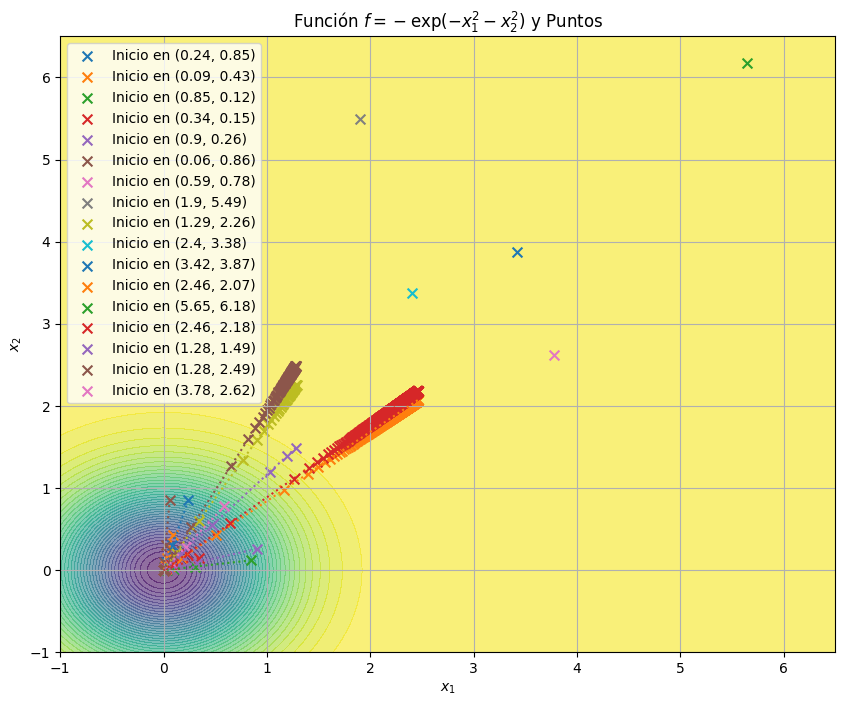
\includegraphics[width=0.65\linewidth]{figuras/PREG8_GRAD.png}   
    \label{fig:enter-label}
\end{figure}

%\begin{itemize}
%    \item Cantidad de iteraciones totales : $14$
%    \item Tiempo de ejecucion :  $0.1810$ seg.
%    \item Punto $x^k$ encontrado : $( 0.000000351529 , 0.000000351529)$
%    \item Tiempo de ejecucion : $0.13$ segundos

%\end{itemize}


\item Utilizando el método de descenso de gradiente con busqueda de Armijo

\begin{table}[H]
\centering
\renewcommand{\arraystretch}{1.2} % Aumenta el espacio vertical entre las filas
\begin{tabular}{|c|c|c|c|c|c|c|c|}
\hline
\textbf{Iter$_{total}$} &\textbf{Des$_{total}$}&\textbf{Arm$_{total}$} & \textbf{x$_{inicial}$}& \textbf{$x^k$} & \textbf{||$\nabla \mathbf{f(x^k)}$}|| & \textbf{f($\mathbf{x^k}$)} & \textbf{tiempo} \\
\hline
15  & 88 &260 & (0.24 , 0.85) &( 0.00000,0.00000 ) & 0.00000079 & -1.00000000 & 4.7337 \\
15  & 77 &228 & (0.09 , 0.43) &( 0.00000,0.00000 ) & 0.00000055 & -1.00000000 & 4.7221 \\
15  & 88 &260 & (0.85 , 0.12) &( 0.00000,0.00000 ) & 0.00000076 & -1.00000000 & 5.8824 \\
14  & 75 &222 & (0.34 , 0.15) &( 0.00000,0.00000 ) & 0.00000093 & -1.00000000 & 4.0884 \\
15  & 82 &241 & (0.9 , 0.26) &( 0.00000,0.00000 ) & 0.00000084 & -1.00000000 & 5.1413 \\
15  & 88 &260 & (0.06 , 0.86) &( 0.00000,0.00000 ) & 0.00000077 & -1.00000000 & 4.2686 \\
15  & 90 &265 & (0.59 , 0.78) &( 0.00000,0.00000 ) & 0.00000089 & -1.00000000 & 4.9996 \\
1  & 1 &0 & (1.9 , 5.49) &( 1.90000,5.49000 ) & 0.00000000 & -0.00000000 & 0.0000 \\
52  & 283 &453 & (1.29 , 2.26) &( 0.00000,0.00000 ) & 0.00000080 & -1.00000000 & 18.3300 \\
1  & 1 &0 & (2.4 , 3.38) &( 2.40000,3.38000 ) & 0.00000029 & -0.00000003 & 0.0000 \\
1  & 1 &0 & (3.42 , 3.87) &( 3.42000,3.87000 ) & 0.00000000 & -0.00000000 & 0.0000 \\
851  & 1537 &1702 & (2.46 , 2.07) &( 0.00000,0.00000 ) & 0.00000065 & -1.00000000 & 180.5773 \\
1  & 1 &0 & (5.65 , 6.18) &( 5.65000,6.18000 ) & 0.00000000 & -0.00000000 & 0.0000 \\
1285  & 1942 &2111 & (2.46 , 2.18) &( 0.00000,0.00000 ) & 0.00000081 & -1.00000000 & 251.5819 \\
18  & 129 &287 & (1.28 , 1.49) &( 0.00000,0.00000 ) & 0.00000084 & -1.00000000 & 5.9728 \\
108  & 436 &598 & (1.28 , 2.49) &( 0.00000,0.00000 ) & 0.00000068 & -1.00000000 & 29.0050 \\
1  & 1 &0 & (3.78 , 2.62) &( 3.78000,2.62000 ) & 0.00000001 & -0.00000000 & 0.0000 \\
\hline
\end{tabular}
\end{table}

\begin{figure}
    \centering
    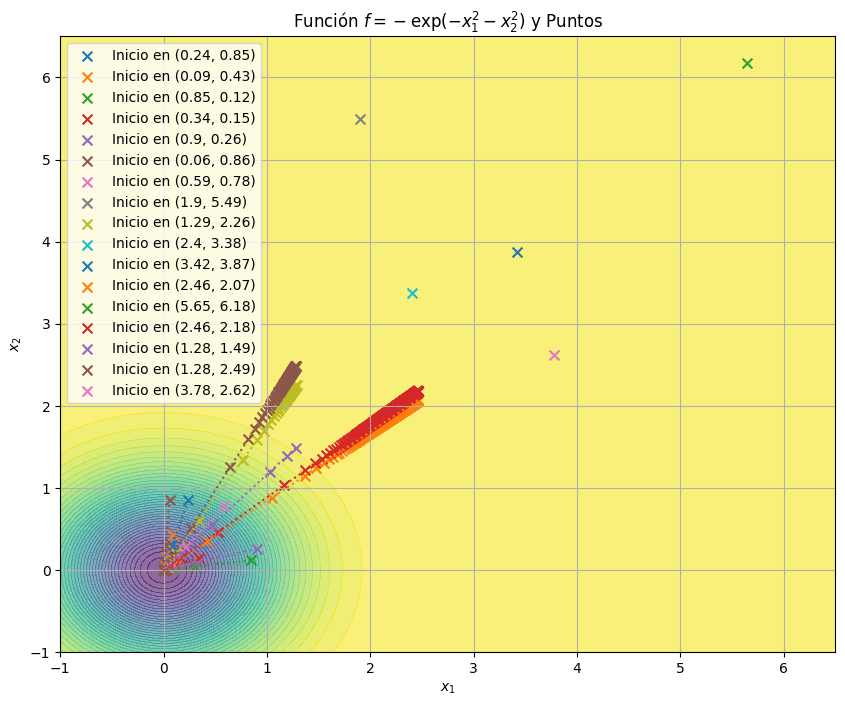
\includegraphics[width=0.65\linewidth]{figuras/PREG8_ARMIJO.png}
    \label{fig:enter-label}
\end{figure}

\begin{itemize}
    \item \textbf{Observaciones del algoritmo :}\\
    En este algoritmo el arreglo de hacer un cambio de la forma \[ x_{k+1} = \quad  arg min \quad \{ f(X)+(1/2) *||X-x^k||^2 \} \] hace posible probar con un punto más lejano a $(0,0)$, para poder encontrar el mínimo $(0,0)$
\end{itemize}
\end{itemize}



